\documentclass[11pt]{article}
\usepackage{EngReport}
\usepackage[acronym,nomain]{glossaries}

\graphicspath{{Images/}}
% \bibliography{Sources.bib}
\microtypesetup{protrusion=false}
\addbibresource{Sources.bib}
\nocite{*}
\makeglossaries
% \onehalfspacing
\setstretch{1.15}
\geometry{letterpaper, portrait, includeheadfoot=true, hmargin=1in, vmargin=1in}

% \fontsize{font size}{vertsize (usually 1.2x)}\selectfont
\fontsize{11}{20}\selectfont{}
\captionsetup{font=footnotesize}

\begin{document}
\renewcommand{\familydefault}{\rmdefault}

\begin{titlepage}
    \begin{center}
    {\fontsize{40}{48}\selectfont \bfseries Cryptography in a Post-Quantum World} 
    \\\vspace{20pt}
    {\LARGE Off to the Races} \\
    \vspace{20pt}
    \textbf{Mason Ballard}
    \vspace{8pt}
    \\ CNT 5412, Fall 2023
    \end{center}

    \bigskip
    \begin{abstract}
       Quantum computing is advancing. Promising speed and power, it has great potential to advance the world we live in while also introducing some new threats. The modern world has become increasing intertwined with the digital world including means of communication, employment, education, public health, commerce, and more. One of the main threats of post-quantum computing is its ability to break current public-key cryptography which in turn could endanger the private information of a great number of people and organizations, important critical infrastructure sectors, and critical infrastructure functions. Though NIST’s updated standards are not expected to be completed and released until 2024, NIST currently has been conducting conferences and calls for papers, choosing algorithms to be standardized and recommended for use as well as collaborating with the NSA and DHS to solicit ideas and research, document decisions, and disseminate recommendations for the public and private sector. The first part of this paper will discuss what quantum computing is with particular attention it’s power within cryptography. Second, we will go over the threats that such increased power will have. Third, we will go over the standards, recommendations, and guidelines in place currently. Because the standardization process is still ongoing we will discuss issues still present to address, the most recent updates gained from research or conferences, and the predicted next steps in this process and it’s forward-looking impact on our world.
    \end{abstract}
\end{titlepage}
\pagestyle{fancy}
\fancyhf{}
\setlength{\headheight}{30pt}
\renewcommand{\headrulewidth}{0.4pt}
\renewcommand{\footrulewidth}{0.4pt}
\lhead{Cryptography in a Post-Quantum World}
\rhead{CNT 5412 - Fall 2023}
\rfoot{\textbf{Page \thepage}}
\lfoot{}

\section*{Summary}
Information is everywhere. It is nearly a currency in our day in age. It covers the frivolous as well as the national critical, and quantum computers have the power to break the systems that currently secure it. In this paper we will discuss the background of quantum computers, the theories on which current work in the field is based, and the current and most recent developments in the field. At the end, we hope you will have a solid foundation and background to join this new ``quantum movement", following the continued updates and discoveries as they come out. 
\pagebreak

\tableofcontents
\pagebreak

\graphicspath{{Images/}}

\section{Introduction}
\subsection{It's an information revolution}
Information is everything. Information is ubiquitous. Information is a name, an email address, an IP address (a digital address), where you live (a physical address), a place of employment, a birthday, a file, a password, a text message, a credit card number, votes in an election, military deployment plans, and more. Information is created everyday, and it is exchanged everyday. It is interwoven with, provides guidelines for, and supports fields and domains that are simultaneously specific and private, owned and affected by the collective, as well as broadly applicable. Information science is a well-established field, and records proving its existence go as far back as the Library of Mesopotamia \cite{30s_history_of_info_science} even though the area of study did not receive its official name until about 1955 \cite{wiki_info_science}. Alan Turing sought to define information science as a ``universal, hardware-independent notion of computation"; whereas, Claude Shannon sought to define information science as a ``universal, meaning-independent notion of communication". Oxford Languages defines \textbf{\gls{info_sci}} as:
    \begin{quote}
        ``a broad and interdisciplinary field that studies how information is created, collected, organized, stored, retrieved, and used by humans and machines. It also examines the social, ethical, legal, and cultural aspects of information and its impact on society." \cite{bing_is_def}
    \end{quote}

\begin{figure}[ht] 
    \centering
    \ffigbox[\FBwidth]
        {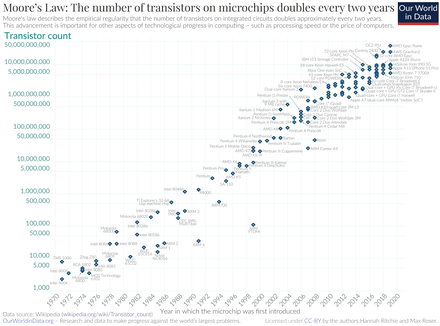
\includegraphics[width=0.65\textwidth]{moores_law.png}}
        {
            \captionsetup{justification=centering}
            \caption{Moore's law is the observation and subsequent prediction the number of transistors per microchip will double every two years}
            \label{fig:moores_law}
        }
\end{figure}

The \textbf{\gls{info_rev}} brought about by the advent of computers and the speed of its growth is quickly summarized using \textbf{\gls{moore}}. Originally published in Electronics Magazine in 1965, Gordon Moore predicted ``the number of transistors per square inch on a microchip would double each year while the manufacturing cost per component would halve" \cite{arcuri_moores}. This was revised a decade later to state ``chip density would...double every two years for at least the next decade
" \cite{arcuri_moores}.

Up until now, Moore's law has quite faithfully remained true, much to Moore's own surprise, made possible because engineers were able to continually develop smaller and smaller transistors. Well-known and regarded as a general rule rather than just a theorem in information science, its veracity has exceeded the predicted ten-year lifetime by more than thirty years as illustrated in Figure \ref{fig:moores_law}, but all good things must come to an end. As of 2016, the smallest transistor yet is roughly the same thickness as a single layer of carbon atoms \cite{yang_transistor}. Sarah Yang from the Berkeley National Lab remarked in ``Smallest transistor ever made by Berkeley Lab" that transistors reaching the atomic scale may be the end of Moore's law as we know it, but maybe the end of one chapter is just the beginning of another. 

\subsection{Time for a quantum revolution: The future is... now?} \label{q_rev}
The study of quantum mechanics goes all the way back to the early 1800s \cite{q_mech_timeline}. Essentially the physics of small things \cite{qc_explained}, the field of quantum mechanics paved the way for the field of quantum computing. When Stephen Wiesner invented conjugate coding in 1965 \cite{qc_timeline}, this marked the beginning of quantum communication and computation and, arguably, a brand new information revolution. Whereas the invention of the classical computer spurred on the growth of the field of information science and provided the foundation for areas of study such as classical communication, computation, and cryptography, the invention of the quantum computer (\textbf{\gls{qc}}) has great promise to do the same.

In an article as recent as October 2023, a quantum computer boasting a record-breaking 1,180 qubits was build by tech startup Atom Computing \cite{atom_computing}. This broke IBM's standing record with their quantum computer, Osprey, having a, what now seems small, 433 qubits (as recent as 2022) \cite{osprey}. In a vein that seems vaguely familiar to Moore's law, this innovation is notable not only because it represents a rapid level of innovation in an unexpectedly short amount of time, this recent news may indicate that quantum computing has the power to usher in new eras of quantum communication, computation, and cryptography in much the same fashion that classical computers kick-started the information revolution beginning in the early 1980s. With quantum computers promising to be more powerful and better at solving complex problems, increased power means great potential to be used for good or bad. 

As an example, Shor's 1994 algorithm promises to be able to effectively do prime factorization with ``strong evidence of super-polynomial speedup" \cite{wiki_shor}. This is significant because the security of many public-key protocols is built on the premise that multiplying two primes is very easy, but given the their product, it is difficult to find it's prime factors especially if these primes were very large. In general, an ideal property for any cryptography scheme to have is that is it easy to compute but difficult to reverse unless you know a secret piece of information, and Shor's algorithm tells us that, backed by the power of quantum computers, public-key protocols used every day by individuals, companies, and world governments for encrypting sensitive and critical data as well as providing digital signatures may be at risk of being broken, leaving the information they protect vulnerable to stealing and exploitation.

\begin{figure}[h] \centering
    \ffigbox[\FBwidth]
        {
            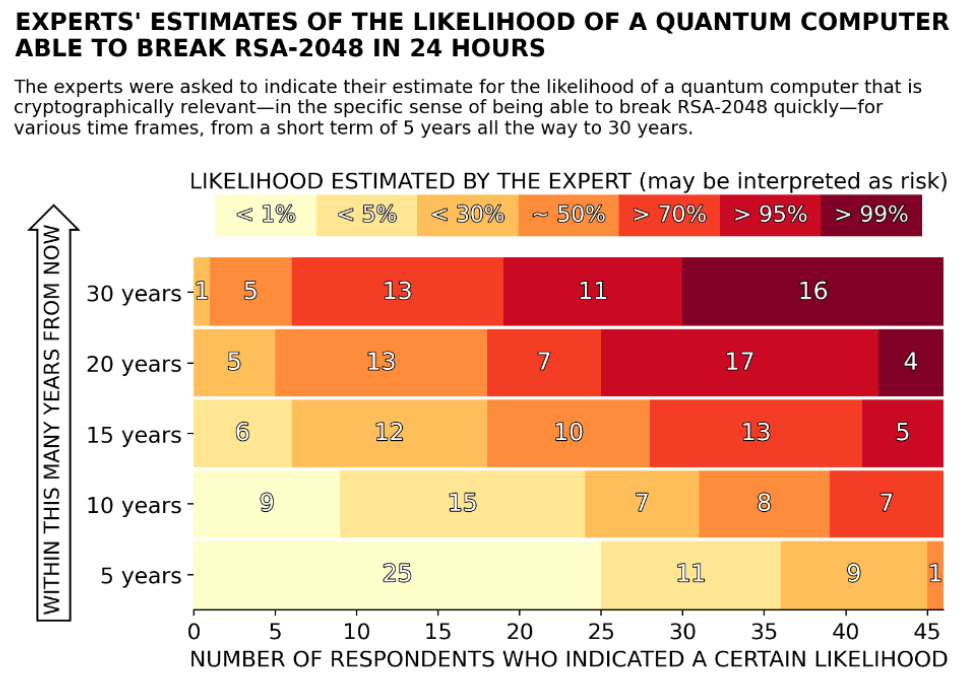
\includegraphics[width=.47\textwidth]{mosca_piani.png}
            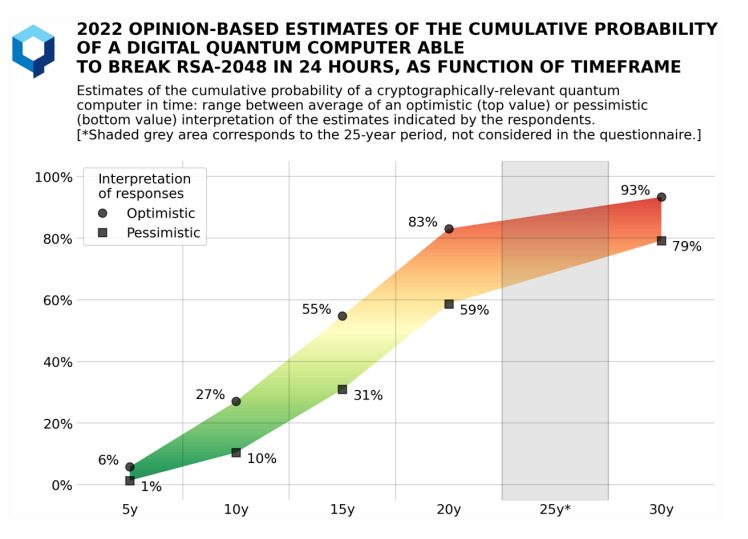
\includegraphics[width=.47\textwidth]{crqc22.png}
        }
        {
            \captionsetup{justification=centering}
            \caption{Mosca and Piani's 2022 survey shows estimates for when a cryptographically-relevant quantum computer may be made range from 5 to 30 years} \label{fig:mosca_piani}
        }
\end{figure}

We have already seen evidence that the quantum field is growing at a rapid pace to say the least. The threat this poses to the current security infrastructure as we illustrated is palpable. If recent developments are any indicator of where the field is going and the cadence it will maintain going forward, it is essential that developments on the defensive security side are worked concurrently, and they must try to keep pace. So far it seems that cryptographers are up to the challenge, and several exciting and interesting discoveries have come out as a byproduct of this work and research. The only question left weighing on many people minds is ``how much time do we have?" which snowballs into other questions such as ``do we have enough time?", ``what can we reasonably expect to accomplish in the time we have?", and ``if we don't have time to do everything we want, what should we prioritize?".

These very questions have received a certain amount of research of their own. Something that may cause anxiety due to the uncertainty of it all or may provide some relief is that computers capable of such computations do not yet exist; however, different researchers have tried to predict when such a computer could be expected, but have come up with answers that range from 5 to 30 years (Figure \ref{fig:mosca_piani}) \cite{mosca_piani_howsoon}. Meanwhile, the US government believes that ``adversarial nation-states are currently investing billions of dollars to weaponize quantum computers" \cite{2022_nsa}. In other words, we aren't entirely sure, but doesn't mean we're clueless. 

\textbf{\gls{moscas_theorem}}, named after renowned mathematician and computer scientist Michele Mosca, gives us a formula by which to judge such questions. More specifically it gives us a formula for us to judge how long we have to find a quantum-safe, -resistant, or -resilient solution and implement it before critical information and systems will be at risk (Figure \ref{fig:moscas_theorem}). \\

    \begin{table}[h]
        \centering
        \begin{tabular}{cl}
     \multicolumn{2}{c}{Given:}\\
             $x \leftarrow$& shelf-life time or how long we need encryption to be secure\\
             $z \leftarrow$& threat timeline or time until large-scale quantum computer is built\\
        \end{tabular}
        \label{tab:mosca_given}
    \end{table}
    
    \begin{table}[h]
        \centering
        \begin{tabular}{cl}
     \multicolumn{2}{c}{We have:}\\
             $y \leftarrow$& migration time or time we have to find a quantum-safe solution and retool existing architecture\\
        \end{tabular}
        \label{tab:mosca_wehave}
    \end{table}
    
    \begin{table}[h]
        \centering
        \begin{tabular}{cl}
     \multicolumn{2}{c}{Which tells us:}\\
             \multicolumn{2}{c}{If $x+y>z$, then it's time to worry!}\\
 \multicolumn{2}{c}{So we need to make sure $y < z-x$}\\
        \end{tabular}
        \label{tab:mosca_worry}
    \end{table}
    
    \begin{figure}[!h]
        \centering
        \ffigbox[\FBwidth]
        {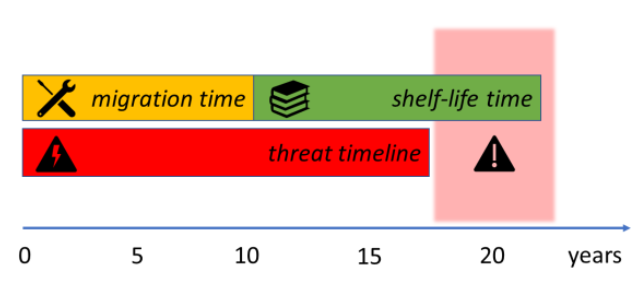
\includegraphics[width=0.65\linewidth]{moscas_theorem.png}}
        {
            \captionsetup{justification=centering}
            \caption{Mosca's theorem gives a mathematical method for conceptualizing the amount of time before quantum resistant/resilient cryptography will be necessary}
            \label{fig:moscas_theorem}
        }
    \end{figure}
    
Mosca's theorem goes hand in hand with a concept becoming increasingly well-known and referenced called a catch-and-exploit attack. In ``Preparing Critical Infrastructure for Post-Quantum Cryptography" written and released by the Cybersecurity and Infrastructure Security Agency \textbf{\gls{cisa}} (an operational component of DHS), a catch-and-exploit campaign is defined as an attack in which ``adversaries capture data that has been encrypted using current encryption algorithms and hold onto such data with the intention of decrypting it when a quantum computer capable of breaking the encryption is available" \cite{cisa_prep4pqc}. This concept is important because it indicates the possibility that once a cryptographically-relevant quantum computer (\textbf{\gls{crqc}}) is made and available data assets may be at risk almost immediately, and it emphasizes the importance of updating the systems that protect and transmit this data as soon as possible. 

The stakes are high, and it is under these circumstances that the US government has banded together to find a solution. While the National Security Agency (\textbf{\gls{nsa}}) searches for possible solutions to protect US National Security Systems (\textbf{\gls{nss}}), the National Institute for Science and Technology (\textbf{\gls{nist}}) has been given the task finding, vetting, and standardizing quantum-safe protocols that could be used to phase out and replace systems currently in use that are most likely to be broken first once quantum computers are widely available. Meanwhile, the Department of Homeland Security (\textbf{\gls{dhs}}) has been tasked with writing and disseminating recommendations for other public sector organizations (\textbf{\gls{fceb}} agencies, \textbf{\gls{sltt}} government organizations) and private sector organizations that provide any of the National Critical Functions (\textbf{\gls{ncf}}s) or support the critical infrastructure (\textbf{\gls{ci}}). 

\subsection{Cryptography in a Post-Quantum World} 
In this paper, we will discuss how the world of cryptography may be affected by the invention and development of quantum computers. This is an introductory discussion; therefore, we will aim to explain broad concepts using simple language. As such, the discussion will not be overly technical, but there are vast resources online which discuss the underlying implementation details, mechanics, and more taught by a variety of individual and organizations ranging from hobbyists to the inventors themselves. We will begin with an explanation of some background topics (Section \ref{quantum_basics}) important to understanding the benefits and limitations of quantum computers. We will then discuss how these basic concepts backed the invention of some foundational systems in quantum cryptography (Section \ref{q_crypto}). We will briefly explain Shor's Algorithm and Grover's Algorithm to understand what they are, why they are important, and how they affect current work in the cryptographic field (Section \ref{shor_grover}). To provide a broad picture of how such work is affecting significant change in our world, we will talk about how the NSA, NIST, and DHS have been working together to secure our future (Section \ref{government}). Post-quantum cryptography standardization is an area of research still very much alive, and there is no better illustration of this than NIST's Post-Quantum Cryptography (\textbf{\gls{pqc}}) Standardization Competition which we will close with in order to give readers the latest update of where the world stands in this development process, what we currently know, and where we predict it will head next (Section \ref{industry}). This discussion will go back and forth between the conceptual and the tangible, leaning more and more heavily on the tangible side of things as we progress. As the discussion becomes more and more tangible and of the moment, we will try to use more and more real life examples to illustrate concepts while remaining introductory friendly. With that, it should be noted that this report cannot with any level of certainty know for sure where and how this industry and this process will conclude or when. We have sourced as many sources as possible within the given time frame to paint a picture of the work and how it currently stands as of the time of writing for the reader. It is our hope is that this paper will provide a good foundation, arming the reader with the knowledge base necessary follow this movement after the writing of this paper, past the initial stages of standardization, and into the growth of the wider industry. Thank you for taking the time, and welcome to the quantum revolution. 

% \redcomm{Hello}
% \greencomm{Hello 2}
% \bluecomm{Hello 3}

% \gls, \Gls, \glspl, \Glspl


\graphicspath{{Images/}}

\section{The Basics of Quantum} \label{quantum_basics}
In its most general form, a quantum computer is a device that stores quantum particles in a controlled environment that is controlled in a such a way that these particles can be made to do what we want \cite{theunlockr}. QCs take advantage of fact that very small particles have unique rules and properties set out by quantum mechanics and quantum physics. In comparison with the properties of larger atoms, quantum particles seem as if they bend the rules of space and time. Acting in a seemingly random manner provable and made a little bit more predictable with mathematical properties and proofs, we use controlled environments with low temperatures, superconducting circuits, fiber optic cables, and more \cite{unc_qc} to control quantum particles like photons in such a way that allows us to do computations on them and use them to solve problems. Where classical computers use bits in distinct zero or one states to store information and use mathematical transformations to do computations and solve problems, quantum computers use quantum bits, referred to as \textbf{\glspl{qubit}}. Some defining properties of qubits that make quantum computers distinct from classical computers are explained below.  

    \subsection{Entanglement}
    The first unique property that quantum particles follow is that of entanglement. It is defined as thus: 
    \begin{quote}
        \textbf{\Gls{entanglement}} is where the quantum state of each particle within a set cannot be described independently of the state of the other particles even when the particles are separated by a large distance. It has been found that position, momentum, spin, and polarization can all be perfectly correlated \cite{entanglement}.
    \end{quote}

    If we imagine qubits as particles that spin, we can compare traditional bits of zeroes and ones to qubits in a spin down state (which correlates to a natural-state of zero) and a spin up state (where this change in energy corresponds to a state of one). Entanglement tells us that given two entangled qubits, if one is spin up, and the relation between them is that they are inverses of each other, the other will be spin down, and if one changes its spin direction the other will automatically change accord to their relation. Additionally, observational research has also shown that entangled qubits are "monogamous" \cite{info_is_quantum}, meaning the more entangled they are with each other, the less they will be with other qubits.
    
    \subsection{Superposition} \label{superposition}
    Imagining qubits in the directly opposing spin up and spin down states, opens the door to discuss in-between states. Schr\"{o}dinger's cat is a thought experiment by Edwin Schr\"{o}dinger introduced in 1935, and it is commonly referenced to explain the idea of superposition:
    
    \begin{quote}
        "A cat, a flask of poison, and a radioactive source are placed in a sealed box. If an internal radiation monitor (e.g. a Geiger counter) detects radioactivity (i.e. a single atom decaying), the flask is shattered releasing the poison which skills the cat. The Copenhagen interpretation [of quantum mechanics] implies that, after a while, the cat is simultaneously alive and dead. Yet, when one looks in the box, one sees the cat either alive or dead, but not both alive and dead." (See Figure \ref{fig:cat}) \cite{schrodinger}
    \end{quote}
    
    \begin{figure}[ht] 
        \centering
        \ffigbox[\FBwidth]
        {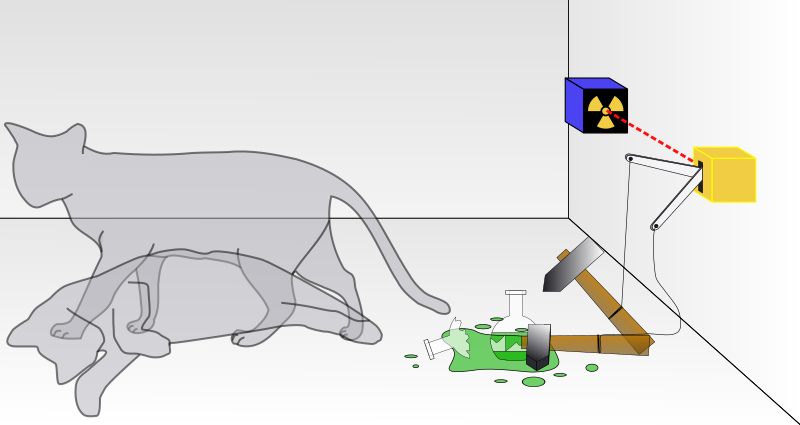
\includegraphics[width=0.65\textwidth]{Schrodingers_cat.png}}
        {
            \captionsetup{justification=centering}
            \caption{"Schr\"{o}dinger's cat: a cat, a flask of poison, and a radioactive source connected to a Geiger counter are placed in a sealed box. As illustrated, the objects are in a state of superposition: the cat is both alive and dead." \cite{schrodinger}}
            \label{fig:cat}
        }
    \end{figure}
    
    Originally intended as a criticism of how insensible the idea of superposition was, it went on to be used as a popular analogy for describing the exact principle it sought to criticize. It then went on to inspire further work that would build upon this premise. Charles Bennett explains the idea of superposition more directly:
    \begin{quote}
        "Between any two reliably distinguishable states in the physical system - not all states or pairs of states are reliably distinguishable - there are intermediate states that are not distinguishable from either one, and they correspond to intermediate directions in space, and the two states are reliably distinguishable if their directions are perpendicular. Any two perpendicular directions correspond to reliably distinguishable states, and any two directions that are not perpendicular correspond to a pair of states that are different but not reliably distinguishable." \cite{charles_b}
    \end{quote}

    Explained as simply as possible, superposition tells us that where a classical computer's bits must be a zero or one, qubits can be many things in between. Not only can it be more than two binary states, superposition tells us that in fact a qubit may be in all possible states at the same time. This increased complexity means that qubit states are often expressed using probabilities in something called \textbf{\gls{ket}} (sometimes referred to as Dirac notation). 

    \subsection{What this means}
    Superposition is the main property that makes quantum computers the ideal tool to evaluate high variable, high complexity problems especially when the problem involves trying to find the best solution from a series of possible sources (an example is the traveling salesman problem) because this property allows us to store and on some level track and represent collective states rather than singular binary states. The one caveat is that reading the state of a quantum system will destroy the superposition information. This is what makes quantum computers not very good at problems that require sorting, possibly performing worse than classical computers. 

    Entanglement is the main property that enabled, inspired, and currently supports the field of quantum communication and its research. It is has inspired schemes such as Bennett and Brassard's BB84 communication protocol, and the way that entangled particles reliably react across long distances has enabled communication schemes that utilize this property to have near instantaneous communication across very large distances.

    Beyond the basic properties of entanglement and superposition, there are a few more basic principles that limit quantum computers. The first property states that no quantum states can be cloned referred to as the no-cloning theorem. Secondly and somewhat relatedly, the exact polarization of a quantum particle or qubit or quantum state cannot be measured. Logically, being able to do one would enable the other and vice versa. These properties have posed issues when it comes to error checking and information transmission fidelity (i.e. what is sent is the same as what is received). Classical computers utilize many different schemes for error checking including parity bits, redundancy checks, and Hamming codes, and many of these involve some level of cloning. As it stands right now, quantum computers are still quite error prone due to the need to created adapted error checking schemes that don't rely on cloning. Multiple schemes have been suggested to combat this, but they have not yet been able to be implemented in a large scale way that would allow us to rigorously test their effectiveness \cite{shor}.









\graphicspath{{Images/}}

\section{Quantum Communication and Cryptography} \label{q_crypto}
If cryptography is the ''art of secret writing'' \cite{netsec}, then \textbf{\gls{q_crypto}} is cryptography that takes advantage of the unique properties of quantum computers to provide \gls{confidentiality}, \gls{integrity}, \gls{non-repudiation}, \gls{authenticity}, and \gls{availability} (see the \gls{cia} in the glossary). If classical computers use mathematical operations to mangle and obscure data, quantum computers use quantum mechanics and physics to do the same. In this way, quantum computers' unique properties allow quantum cryptography to have built in security in ways not possible and more reliable than for cryptography done with classical computers. For example, the no-cloning theorem makes error checking and correction difficult, but it also makes quantum communication more secure.  More generally, \gls{crypto} is:

\begin{quote}
    ``the ability to send information between participants in a way that prevents others from reading it.'' \cite{netsec}
\end{quote}

 To illustrate how cryptography can be made more secure using quantum computers rather than classical computers, we will introduce two common attack vectors that affect both classical and quantum cryptography, then we will use a basic quantum communication protocol to show how quantum computing can be more effective at defending against these vectors.

    \subsection{Common Attack Vectors}
    An \textbf{\gls{attackvector}} is:
    \begin{quote}
        ``the method or combination of methods that cybercriminals use to breach or infiltrate a victim's network'' \cite{attackvectors}
    \end{quote}
    Attack vectors may be individual means of accessing a network or it may be a set of tools and techniques combined to do so. Many attack vectors may be used as introductory or intermediary steps of getting into a system which means they may provide a means of compromising more security objectives than the immediate attack vector itself does.  
    
    \subsubsection{\textbf{\Gls{eavesdropping}}}
    Eavesdropping describes an attack where an adversary may intercept communication. It is a passive attack meaning that the information stream is not modified in any way. However, such an attack does violate the security objective of confidentiality.
    
    \subsubsection{Man-In-The-Middle (\textbf{\gls{mitm}})}
    A man-in-the-middle attack (or meddler-in-the-middle attack) is the active form of eavesdropping wherein an adversary may alter the information stream. They may ``transmit their own messages, replay old messages, modify messages in transit, or delete or delay selected messages in transit'' \cite{netsec}. Because this attack involves an adversary reading and altering information not meant for them, it violates the security objectives of confidentiality and integrity.

    \subsection{Quantum Key Distribution (\textbf{\gls{qkd}})}
    The quantum key distribution method is a secure cryptographic communication protocol which allows participants to generate a shared key. This shared key may be used to privately negotiate an encryption scheme or as a one-time pad (see glossary \textbf{\gls{otp}}). Similar to the previously mentioned BB84, it is based on two principles: the \gls{uncertainty} (see glossary) and the quantum property of entanglement. It works in this way:
    
    \begin{table}[h!]
        \begin{tabular}{cl}{Given:} \\
             $A \leftarrow $ & the sender of some secret information\\
             $B \leftarrow $ & the receiver of some secret information \\
        \end{tabular}
        \label{tab:given_vars}
    \end{table}

    \begin{algorithm}
        \caption{The QKD Procedure is as follows:}
        \label{alg:qkd}
        \begin{algorithmic}[1]
            \Procedure{QKD}{$A$, $B$}
                \State $bits_{sent} \gets \Call{SendBits}{bits_A, Filter_A}$
                \State $Filter_B \gets \Call{rand}{Filters}$
                \Comment{where $Filters$ is a set of filters}
                \State $bits_B \gets \Call{ReceiveBits}{bits_sent, Filter_B}$
                \State $key_{AB} \gets \Call{Compare}{Filter_A, Filter_B}$ \label{compare}
            \EndProcedure
        \end{algorithmic}
    \end{algorithm}

    In this procedure, $A$ sends some bits through a polarizing filter (see Appendix \ref{note:polarize}) to $B$. Because $B$ doesn't know which polarizing filters $A$ used, they use a random set of filters to receive these bits through. Once A has finished sending these bits and B has finished receiving them, they compare the polarizing filters they used. They keep the bits sent/received that match and discard those that do not. This set of matching bits becomes the shared key. Now, how does this protect against eavesdropping or MITM attacks?

    \subsubsection{Protecting Against Eavesdropping and MITM Attacks}
    An adversary could try to listen in on the communication between $A$ and $B$, but reading a state destroys the superposition information which effectively changes the state. An adversary could try to use their own polarizing filter to read and/or pass on the information transmitted, but without being to compare (step \ref{compare}), any information they collect is somewhat useless. Even better than the fact that an outsider is not able to effectively listen in or manipulate information communicated using this protocol is the way that doing so alters the information stream in a way that very quickly alerts the communicating parties that there is some interfering force that is not supposed to be there. This ability to protect against and detect any attempted meddling means that communicating parties can quickly and effectively respond (i.e. starting over), and they can rest assured that future communication will be secure from having been breached at this initial stage. 
\graphicspath{{Images/}}

\section{Breaking Classical Cryptography} \label{shor_grover}
Just as quantum communication and cryptography developed to utilize quantum computers for better communication and security, the offensive side of computer security was able to take advantage of the unique properties of quantum computers to perform better as well\footnote{Defensive cryptography typically refers to systems, protocols, and schemes used to protect sensitive information from outside forces while the term offensive security is typically used to refer to cryptographic systems, protocols, and schemes that attack, break, or take advantage of weaknesses in systems to gain access to valuable and sensitive information. Though it may sound like one is a good thing and one is a bad thing, both work together and are equally important to make sure the systems that protect information grow with the industry that surround them.}. Two algorithms that exemplify this growth and how it can cause a domino effect on the industry and the world by extension are \textbf{\gls{shor}} and \textbf{\gls{grover}}.

    \subsection{Shor's Algorithm}
    Shor's algorithm was made by Peter Shor in 1994. Inspired by Dan Simon's research discussing an oracle function\footnote{a "black box" function that when given an input gives an output; the implementation of how such a task might be done may not be known, but such a concept is often in proofs to provide abstract concepts not yet realized that may allow other discoveries} capable of finding a period\footnote{a point at which a cyclical group repeats\label{period}} as well as taking advantage of the observation that Fourier transformations\footnote{a function capable of decomposing a waveform; implementation not relevant to this discussion} are good at find periodicity, Shor was able to devise an algorithm capable of breaking the discrete log problem and later developed this algorithm further to accomplish prime factorization with a super-polynomial speedup (when compared with classical algorithms; previously mentioned in Section \ref{q_rev}) \cite{shor}. 
    
    \subsection{Grover's Algorithm}
    Grover's algorithm was made by Lov Grover in 1996. It is a search algorithm designed for use on unstructured datasets. Given a black box that produces a unique output, Grover's algorithm can find the unique input that produced this output with high probability. If the function's domain size is $N$, Grover's algorithm can find such an input with only $O(\sqrt{N})$ evaluations.

    \subsection{Why does this matter?}
    As previously discussed, Shor's algorithm can be used to break many if not nearly all public-key cryptography systems. This includes:
    \begin{itemize}
        \item the Diffie-Hellman key exchange
        \item ElGamal public-key encryption
        \item the Digital Signature Algorithm (\textbf{\gls{dsa}})
        \item Elliptic Curve Cryptography (\textbf{\gls{ecc}} which includes Elliptic Curve Diffie-Hellman)
        \item the Rivest-Shamir-Adleman (\textbf{\gls{rsa}}) encryption protocol
    \end{itemize}

    While Grover's algorithm could:
    \begin{itemize}
        \item optimize \textbf{\glspl{bruteforceattack}}
        \item find collisions in hash-based systems, acting as a precursor for \textbf{\gls{preimageattack}}
    \end{itemize}

    Currently Grover's algorithm has several restrictions that limit its implementation and use. One of these is that it is designed for use on unstructured datasets. The second is that it only provides a quadratic search speedup rather than, for example, an exponential one. When applied to structured datasets or smaller datasets, this algorithm may actually be less efficient or slower than other schemes such as the parallel rho algorithm\footnote{used to solve the elliptic curve discrete log problem } \cite{gill_ecc}\cite{grover_no_adv}.

    Neither algorithm has a quantum computer in existence able to run them with a low enough margin of error to be useful.

    As you can see quantum computing, communication, and cryptography are growing on both the defensive and offensive side, and we know that Mosca's theorem put together with current predictions for when a cryptographically-relevant quantum computer could be expected tells us that now is as good a time as any to start preparing and strengthening current systems for its arrival. 
\graphicspath{{Images/}}

\section{Collaborating for Public Reform} \label{government}
In 2015, the \gls{nsa}'s Information Assurance Directorate (IAD) announced that they would ``initiate a transition to quantum resistant algorithms in the not too distant future" \cite{moody_lets_2018}. Ditching their current initiative at the time called Suite B, they stated that they would be searching for ``cost-effective security against a potential quantum computer" \cite{2022_nsa}. Stating that it must be cost-effective indicated that this new solution must be compatible with a wide variety of systems already in use. It is also one of the reasons that the NSA recommended pursuing research and searching for solutions in Post-Quantum Cryptography (\gls{pqc}) rather than Quantum Key Distribution \gls{qkd} systems\footnote{post-quantum cryptography is cryptography not weakened or completely broken by Shor or Grover's algorithm while being suitable for a wide range of applications; quantum key distribution in comparison is best for point-to-point communication \cite{ee_web}}.  

This is the announcement that inspired \gls{nist} to kick off their Post-Quantum Cryptography Standardization Competition which we will discuss in the next section.

The original plan was that the NSA would work to secure the National Security Systems (\gls{nss}) since they fell under the NSA's domain of responsibilities while NIST would work toward standardizing protocols and schemes that could be used and recommended to other government organizations and broader industry. However, because President Biden's January 2022 National Security Memorandum (\textbf{\gls{nsm}}-8) gave the NSA 180 days to ``identify instances of encryption used on NSS not in compliance with NSA-approved quantum resistant algorithms, as well as provide a plan and timeline to transition those systems to quantum resistant standards" \cite{2022_nsa}, this plan had to pivot to accommodate this shortened timeline. 

As a result NIST continued to pursue their PQC Standardization Competition, while the NSA joined forces with DHS to find an intermediary solution as well as draft and disseminate a plan that could be recommended to FCEB, SLTT, CI, and some private industry organizations and vendors. 

Fulfilling their part of the deal, DHS's CISA has released multiple white papers\footnote{refers to an information publication made available to the public, i.e. it is not confidential or restricted} that educate, make recommendations, and update industry leaders as well as the public. Recommendations in these papers (specifically ``Preparing Critical Infrastructure for Post-Quantum Cryptography" released in 2022) include things like:
\begin{itemize}
    \item creating a "post-quantum readiness roadmap" and encouraging vendors and service providers that work with the organization to do the same
    \item putting together a project management team to "plan and scope the organization's migration to PQC" , including the organizations "cybersecurity and privacy risk managers who can prioritize assets that would be most impacted by a CRQC and/or would expose the organization to greater risk" 
    \item developing an inventory of vulnerable and dependent systems with the cooperation of information technology and operational technology procurement experts, engaging with supply chain vendors to identify these technologies (much in the same mentality as developing a Software Bill of Materials (see \textbf{\gls{sbom}} in glossary))
    \item prioritizing high impact systems, industrial control systems (\textbf{\glspl{ics}}), and systems with long-term confidentiality/secrecy needs
    \item identifying data reliant on quantum vulnerable technologies, either updating these systems or coming up with plans and/or timelines to phase them out
    \item engaging with vendors on their roadmap to clarify when and how each commercial-off-the-shelf (\textbf{\gls{cots}}) vendor ``plans to deliver updates or upgrades to enable the use of PQC, as well as the expected cost associated with" such a migration
    \item engaging with cloud service providers to ``understand the provider's quantum-readiness roadmap" 
\end{itemize}

This quantum revolution, its increased capabilities as well as its increased threats has encouraged cross collaboration on every level. We have illustrated how the collaboration between the NSA and DHS has enacted change, and next we will discuss the last piece of the puzzle: how NIST is using their PQC Standardization Competition to find algorithms to standardize for use in both the private and public sector.
\graphicspath{{Images/}}

\section{NIST's PQC Standardization Competition} \label{industry}
In 2009, NIST published a PQC survey, but it wasn't until 2012 that they announced the PQC competition. Spurred on by the announcement made by the NSA that the US government systems would be pursuing quantum-safe solutions, NIST published a report on PQC (\textbf{\gls{nistir}} 8105), devised a timeline, a series of submissions criteria, as well criteria by which to judge and test submissions. The rules and guidelines of the competition were presented at the PQCrypto Conference in 2016 in Japan with the caveat that such standards and rules may shift and change with input from the community. No stranger to competitions, NIST has successfully used similar competitions to standardize 
    the Diffie-Hellman and Elliptic Curve Diffie-Hellman protocol (\textbf{\gls{ecdh}})(which resulted in \textbf{\gls{sp}} 800-56A),
    the RSA encryption scheme (SP 800-56B, \textbf{\gls{fips}} 186),
    DSA and Elliptic Curve DSA (\textbf{\gls{ecdsa}})(FIPS 186), 
    and more.
All of these past standards however were liable to be vulnerable to attack should a CRQC become available, and despite the familiarity of the process of standardizing new algorithms or updating standards for algorithms already in existence, the task of finding post-quantum algorithms to standardize and recommend was a much larger task that before because 
    (1) post-quantum cryptography was going to be more complicated than the cryptography required for past competitions, 
    (2) there would be no ``silver bullet" because all algorithms would have benefits and weaknesses (NIST stated in addition they'd ideally like to choose more than one ``winner"), 
    (3) the algorithms chosen must be able to work on a wide variety of systems, and 
    (4) they must be able to be run and be tested on classical systems while being quantum-safe. 

\begin{figure}[h] 
    \centering
    \ffigbox[\FBwidth]
        {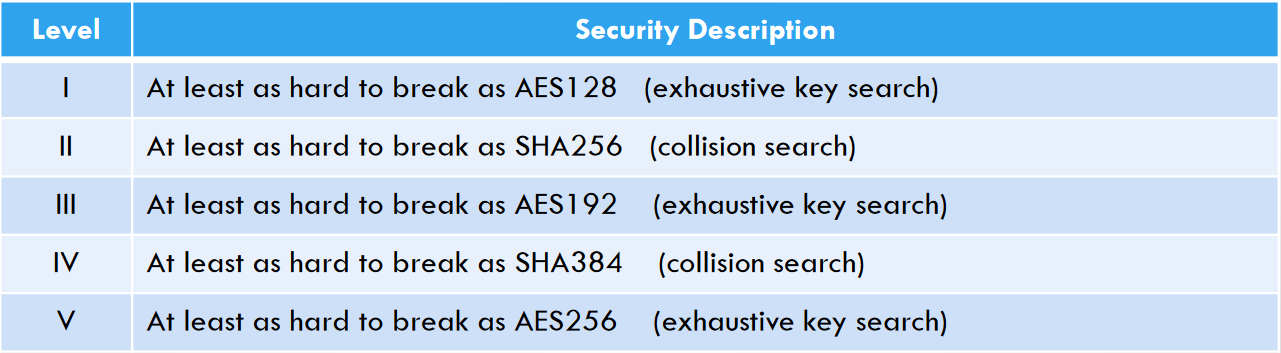
\includegraphics[width=0.75\textwidth]{security_lvls.png}}
        {
            \captionsetup{justification=centering}
            \caption{NIST's levels of security on which algorithms would be graded}
            \label{fig:sec_levels}
        }
\end{figure}

Included in this announcement, they stated that they would be looking for digital signature, encryption, and key exchange algorithms (\textbf{\glspl{kem}}) (while not being part of the official competition, they later announced that they would be looking for proposals for stateful hash-based signature algorithms as well). They expressed the desire for algorithms that would cover these three bases while being based on a variety of different types of quantum algorithms. In their solicitation for proposals and papers, they stated that submissions should be publicly disclosed and freely available, having signed statements with patent information disclosed, having ``theoretical and empirical evidence providing justification for security claims", and including ``concrete...parameters for meeting target security levels" (see Figure \ref{fig:sec_levels}) \cite{moody_ship_sailed}.

In addition to security, they stated that algorithms would be judged on performance. Algorithm capable of additional features would be considered even better. Examples of additional features that NIST was looking for included:
\begin{itemize}
    \item``drop-in replacements - compatibility with existing protocols and networks,
    \item perfect \textbf{\gls{forwardsecrecy}},
    \item resistance to \textbf{\glspl{sidechannelattack}},
    \item simplicity and flexibility,
    \item misuse resistance" \cite{moody_fourth},
    \item and any other additional features similar to those already stated
\end{itemize}

In a presentation given by Dustin Moody (NIST Fed) at the AsiaCrypt conference in 2017, NIST described their role as ``managing a process of achieving community consensus in a transparent and timely manner" \cite{moody_ship_sailed}.

\subsection{Off to the Races}
In the initial set of submissions, NIST received 82 papers with 69 papers meeting the minimal submissions criteria, being considered "complete and proper" \cite{moody_lets_2018}. Round over round and year after year, progress marked by continued presentations, workshops, and conferences whittled the number of algorithms in the running down quickly. Algorithms were eliminated for a variety of reasons such as being broken, significantly attacked, NIST lacking full confidence in their security, or the algorithms being deemed too inefficient. There were small alterations to submissions criteria and judging criteria made to incorporate feedback from the community and introduce a bit more flexibility. Some submissions were added in later rounds while other similar ones were merged, and some submissions were given suggestions to make improvements into order to move forward in the competition. As is illustrated in Figures \ref{fig:algossorted} and \ref{fig:algosbreakdown}, there were a variety of algorithms for encryption and key exchange as well as signatures which were split into several categories based on the type of quantum algorithm they utilized. By the end of the third round in 2022, four algorithms had been chosen for standardization: one lattice-based encryption/key exchange protocol, two lattice-based\footnote{refers to the type of quantum algorithm used, namely, it refers the quantum physics property or scheme that allows an algorithm built on it to be secure} \footnote{types of quantum algorithms include: 
(structured and unstructured) lattice-based (module learning with errors, module learning with rounding), isogeny based, code-based (Goppa, short Hamming, low rank), symmetric-based, hash-based, multivariate-based schemes, and more.} digital signature schemes, and one hash-based digital signature scheme. A quick summary of each is given as follows:

\begin{figure}
    \centering
    \ffigbox[\FBwidth]
        {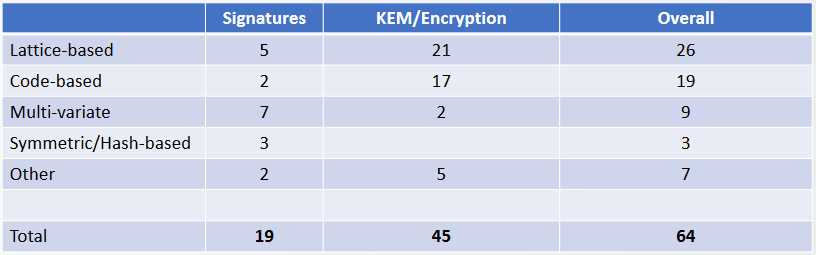
\includegraphics[width=0.65\textwidth]{algosbreakdown.png}}
        {
            \captionsetup{justification=centering}
            \caption{The breakdown of algorithms submitted in the first round. The majority were lattice-based encryption/key exchange protocols \cite{moody_lets_2018}}
            \label{fig:algosbreakdown}
        }
\end{figure}
\begin{figure}
    \centering
    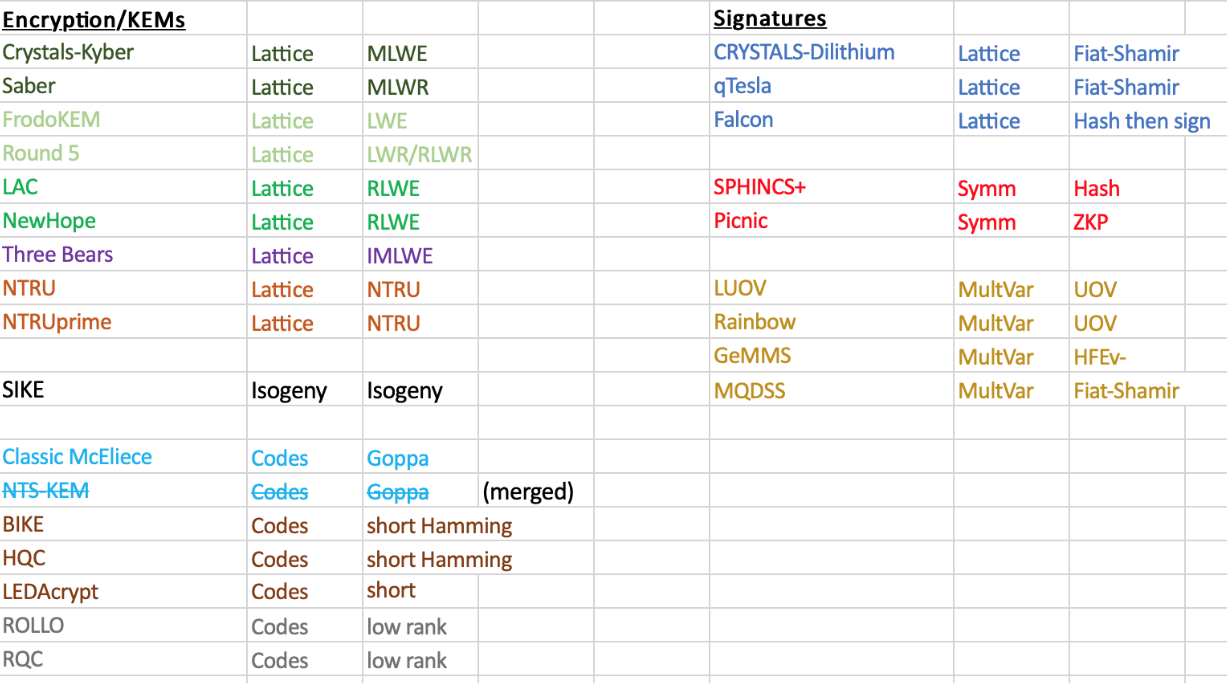
\includegraphics[width=0.75\linewidth]{Images/algos_sorted.png}
    \caption{The list of second round candidates sorted by algorithm type \cite{moody_round2}}
    \label{fig:algossorted}
\end{figure}

\subsection{CRYSTALS-Kyber}
The only public-key encryption/key exchange protocol chosen for standardization at the end of the third round was CRYSTALS-Kyber which was based on structured lattices and the module learning with errors problem. Designed to have IND-CCA2\footnote{indistinguishability under adaptive chose ciphertext attack} 
base level security when used for key exchange and IND-CPA\footnote{indistinguishability under chosen plaintext attack} 
base level security when used for encryption, it was chosen for its ``strong security and performance" \cite{moody_fourth}. NIST stated they would standardize sub-schemes Kyber-768 (providing level 3 security, see Figure \ref{fig:sec_levels}) and Kyber-1024 (providing level 4 security), and they were considering standardizing Kyber-512 as well (at the time of the fourth round they stated that this was just barely meeting level 1 security but it could be advantageous to standardize due to the current cost, stating it would be offered as a smaller alternative). This culminated in Draft FIPS 203 released August 24, 2023 which closed its public comment period on November 22, 2023.

\subsection{CRYSTALS-Dilithium}
One of the two structured lattice-based digital signature schemes chosen for standardization was from the same team as CRYSTALS-Kyber. CRYSTALS-Dilithium used a ``Schnorr-like" \cite{dilithium} lattice-based scheme, supported by the module learning with errors problem. It was chosen for its "strong security and performance", and NIST stated that they planned to standardize the parameter sets that corresponded with ``security categories 2, 3, and 5" \cite{moody_fourth}. This culminated in Draft FIPS 204 released August 24, 2023 which also closed its public comment period on November 22, 2023. 

\subsection{Falcon}
Falcon is the second of the two structured lattice-based digital signature schemes and third of the overall schemes chosen for standardization. It was chosen for standardization as a possible alternative for applications where the CRYSTALS-Dilithium signature was too large. When the team behind Falcon were tasked with presenting their scheme they laid out how their scheme is different, its strengths, its weakness, as well as some ideal applications. Falcon is the only scheme that uses floating point arithmetic and as such must be run on systems with floating point units (\textbf{\gls{fpu}}). This could pose a limitation on its adoption in the case of devices without FPUs, with FPU emulators, or variable-time FPUs. Where systems use emulators or variable-time FPUs, the performance of Falcon may be slower or less reliable, and for companies trying to keep the scheme they use secret, Falcon would not be the best choice because of its unique implementation. The team described vehicle-to-vehicle communications, TLS certificates, systems that don't have a lot of resources for verification, and DNSSEC\footnote{Domain Name System Security Extensions} as ideal applications. NIST announced that they would write the draft standard document for Falcon after completing those for Kyber, Dilithium, and SPHINCS+ which means that despite not having been published yet, such a draft document for which a public comments period will open is due any day now. 

\subsection{SPHINCS+}
SPHINCS+ is the final scheme chosen for standardization thus far, and it is the only hash-based digital signature scheme chosen for standardization. Chosen for its ``solid security", it was originally listed as an alternate when the finalists were announced during the third round; however, the premise which its security is based has existed long enough to have made SPHINCS+ a safe bet. As such, this resulted in Draft FIPS 205 which closed its period for public comments November 22, 2023.

\subsection{The Fourth Round...}
As it currently stands, the PQC Standardization Competition is technically in its fourth round. As mentioned before three draft FIPS documents have been released, and we are awaiting a fourth for Falcon. NIST announced additional public key encryption/key exchange protocols BIKE, Classic McEliece, HQC, and SIKE will be candidates further considered for standardize. They have also released a call for proposals for digital signature algorithms with short signatures and fast verification \cite{announcingfourth}. 

\subsection{... Moving Forward}
The fifth PQC standardization conference is scheduled to be held April 10-12, 2024. On their website they state the purpose will be to ``discuss various aspects of the algorithms (both those selected and those being evaluated) and to obtain valuable feedback for informing decisions on standardization" \cite{announcingfifth} where representative from all teams creating algorithms under consideration will present. When the competition was initially announced, NIST stated that they would like to release standard by 2023. Halfway through the competition they received recommendation that they take their time to ensure a thoughtful and thorough evaluation process. When this decision was made, they amended their statement to say that standards would be available sometime in 2024. The process of not only finding solutions but making sure that the solution found are diverse and robust is an ongoing process which NIST is taking very serious. Coordinating a process in which scientists, mathematicians, physicists, as well as many other types of researchers from all over the world are participating in is a large task to take on, but it has been redeeming to see the ways in which people have come together to create solutions. The process of post-quantum standardization is likely to be an ongoing task that will not end very soon and may not end necessarily when quantum computers arrive. It is much more likely that the coming of a CQRC will create as much if not more excitement, presenting new challenge, we have seen from the discussion of the possibility of one which prompted the PQC competition. It is unclear where this timeline will end, but there have been many promising development to have come out of it. 
\graphicspath{{Images/}}

\section{Conclusion}
Information makes up the threads that tie us together in this world and supports us as we move forward; therefore, the threat of a quantum computer capable of breaking the system that protect this information was a cause of great concern. Its unclear when such a computer will exist, and the power that a quantum computer may provide is only just started to be uncovered. With great potential and also posing great risk, we have seen individuals as well as government come together to find solutions that cross countries and backgrounds. This initial standardization phases is not over. We do not yet have a quantum computer to effectively test if they are fully secure and if they are, how long they will be so. Its too early in this ``quantum revolution" to be able to tell how rapidly the field will grow. There is a whole world cryptography that could developed with quantum computers yet untapped. Beyond the codification and standards, it is yet to be delved into the possible applications for quantum computers though theoretical ideas do exist. Uncertainty can invite fear, but there is also a very high ceiling for potential which we are only just beginning to explore. Healthy curiosity and teamwork has brought us here, and maybe these pieces are exactly what we need to keep moving forward.
    
\pagebreak\pagebreak

\fontsize{9}{12}\selectfont{}
\singlespacing
\graphicspath{{Images/}}

\fontsize{9}{12}\selectfont{}
\singlespacing

\section{Appendix}
    \subsection{Glossary}
    \newglossaryentry{info_sci}{name=information science, description={- the study and practice of how to "collect, store, retrieve, and use information effectively"; explores the "social, ethical and cultural aspects of information"; combining "concepts and methods from various disciplines such as library science, computer science, linguistics, and psychology" \cite{bing_info_science}}}
    
    \newglossaryentry{info_rev}{name=information revolution, description={- "the radical changes wrought by computer technology on the storage of and access to information since the mid-1980s" \cite{info_rev}}}

    \newglossaryentry{moore}{name=Moore's law, description={- "the observation that the number of transistors in an integrated circuit... doubles about every two years" \cite{moore}}}
    
    \newacronym{nsa}{NSA}{- National Security Agency}
    
    \newacronym{nss}{NSS}{- National Security Systems; "systems that contain classified information or are otherwise critical to military or intelligence operations" \cite{nsm_10}}
    
    \newacronym{nist}{NIST}{- National Institute for Standards and Technology}
    
    \newacronym{dhs}{DHS}{- Department of Homeland Security}
    
    \newacronym{qc}{QC}{- quantum computer}
    
    \newacronym{pqc}{PQC}{- post-quantum cryptography}

    \newglossaryentry{moscas_theorem}{name=Mosca's theorem, description={- a theorem created by Michele Mosca that gives a "quantum threat timeline [to determine] whether a cyber-system is already at risk, well before the quantum threat has become concrete, because one has also to consider the needed migration time and the desired or required (e.g. by regulations) shelf-life time" \cite{quantum_threat_timeline}}}
    
    \newacronym{cisa}{CISA}{- Cybersecurity and Infrastructure Security Agency; an operational component of DHS}
    
    \newacronym{crqc}{CRQC}{- a cryptographically relevant quantum computer; a computer "capable of actually attacking real world cryptographic systems that would be infeasible to attack with a normal computer" \cite{nsa_pqc_faq}}
    
    \newacronym{ncf}{NCF}{- national critical functions; "functions of government and the private sector so vital to the United States that their disruption, corruption, or dysfunction would have a debilitating effect on security, national economic security, national public health or safety, or any combination thereof" \cite{ncfs}}
    
    \newacronym{fceb}{FCEB}{- Federal Civilian Executive Branch; often used to refer to ".gov" agencies}

    \newacronym{sltt}{SLTT}{- State/Local/Tribal/Territorial}

    \newacronym{ci}{CI}{- critical infrastructure}

    \newglossaryentry{entanglement}{name=entanglement, description={- the quantum state of each particle within a set cannot be described independently of the state of the other particles even when the particles are separated by a large distance; position, momentum, spin, and polarization may be all perfectly correlated \cite{entanglement}}}

    \newglossaryentry{qubit}{name=qubit, description={- a quantum bit}}

    \newglossaryentry{ket}{name=bra-ket notation, description={- sometimes referred to as Dirac notation, this is a special notation used in quantum mechanics to describe quantum states; its unique representation allows us to "compute probabilities, transition amplitudes, and other important quantities in quantum mechanics" \cite{dirac}}}

    \newglossaryentry{cia}{name=CIA triad, description={- the CIA triad defines the three key security objectives in cryptography; these are \gls{confidentiality}, gls{integrity}, and \gls{availability}; additional objectives of \gls{non-repudiation} and \gls{authenticity} are often considered sub-objective of integrity}}

    \newglossaryentry{confidentiality}{name=confidentiality, description={- information should not be divulged to unauthorized parties; only entities with express or explicit permission should be able to access information}}
    
    \newglossaryentry{integrity}{name=integrity, description={- information must not be modified or destroyed by outside parties or without authorization; sender and receivers of information should be able to trust the information sent or received has not and will not be tampered with or altered}}
    
    \newglossaryentry{non-repudiation}{name=non-repudiation, description={- actions should be uniquely traceable to the person or entity that did it}}
    
    \newglossaryentry{authenticity}{name=authenticity, description={- an entity is who they say they are; data has come from a trusted source}}
    
    \newglossaryentry{availability}{name=availability, description={- a system is available for use when needed and requested; can refer to timeliness and reliability}}

    \newglossaryentry{crypto}{name=cryptography, description={- the ability to send information between participants in a way that prevents others from reading it}}
    \newglossaryentry{q_crypto}{name=quantum cryptography, description={- cryptography that uses quantum mechanical phenomena to secure communication \cite{wiki_qcrypto}}}

    \newglossaryentry{attackvector}{name=attack vector, description={- "the method or combination of methods that cybercriminals use to breach or infiltrate a victim's network" \cite{attackvectors}}} 

    \newacronym{qkd}{QKD}{- quantum key distribution}

    \newglossaryentry{eavesdropping}{name=eavesdropping, description={- a passive attack where an adversary listens in on a information stream}}
    
    \newacronym{mitm}{MITM}{- a man-in-the-middle attack; an active attack where an adversary may "transmit their own messages, replay old messages, modify messages in transit, or delete or delay selected messages in transit" \cite{netsec}}

    \newacronym{otp}{OTP}{- one-time pad; a "single-use pre-shared key larger than or equal to size of the message being sent" that provides perfect secrecy, meaning it is technically impossible to crack \cite{wiki_otp}}

    \newglossaryentry{uncertainty}{name=Heisenberg uncertainty principle, description={- sometimes called the indeterminacy principles, it states "there is a limit to the precision with which certain pairs of physical properties, such as position and momentum, can be simultaneously known' \cite{uncertainty}}}

    \newacronym{dsa}{DSA}{- Digital Signature Algorithm}
    \newacronym{ecdsa}{ECDSA}{- Elliptic Curve Digital Signature Algorithm}
    \newacronym{ecdh}{ECDH}{- Elliptic Curve Diffie-Hellman}
    \newacronym{ecc}{ECC}{- Elliptic Curve Cryptography}
    \newacronym{rsa}{RSA}{- Rivest-Shamir-Adleman; an asymmetric encryption algorithm}

    \newglossaryentry{bruteforceattack}{name=brute-force attack, description={- an attack where an adversary tries all possible inputs to try to break into a system; on average, they must try about fifty percent before (i.e. passwords) before succeeding}}

    \newglossaryentry{preimageattack}{name=pre-image attack, description={- an attack where an attack tries to find a message which hashes to a specific value}}

    \newacronym{nsm}{NSM}{- National Security Memorandum}
    
    \newacronym{ics}{ICS}{- industrial control systems}
    
    \newacronym{cots}{COTS}{- commercial-off-the-shelf}

    \newacronym{sbom}{SBOM}{- Software Bill of Materials; likened to a ingredients list on a food label or receipt from the grocery store, this is an itemized and nested list of items that make up a software component that could be maintained for a vendor or given to potential consulting and contracting customers when building products, tools, and systems}

    \newglossaryentry{schrodinger}{name=Schr"\{o\}dinger's cat, description={- a thought experiment developed by Edwin Schr"\{o\}dinger in 1935 to criticize the Copenhagen interpretation of quantum mechanics; used to describe the quantum property of superposition, this scenario describes "a cat, a flask of poison, and a radioactive source connected to a Geiger counter" are placed in a sealed box, and until the box is opened, the cat may be both alive and dead at the same time}}
    
    \newglossaryentry{shor}{name=Shor's algorithm, description={- an algorithm devised by Peter Shoe in 1994 that is able to break the discrete log problem as well as the prime factorization problem}}
    
    \newglossaryentry{grover}{name=Grover's algorithm, description={- an algorithm devised by Lov Grover in 1996 capable of finding a unique input that was given to black box function when given its unique output, searching unstructured datasets with a polynomial speedup}}

    \newacronym{nistir}{NISTIR}{- NIST Interagency Report}
    
    \newacronym{aes}{AES}{- Advanced Encryption Standard}
    
    \newacronym{sha3}{SHA-3}{- Secure Hash Algorithm 3; an improved and more secure version of the SHA protocol}
    
    \newacronym{fips}{FIPS}{- Federal Information Processing Standards}
    \newacronym{sp}{SP}{- Special Publication}
    \newacronym{kem}{KEM}{- key encapsulation method; a method used "to secure symmetric key material for transmission using asymmetric (public-key) algorithms" \cite{wiki_kem}}

    \newglossaryentry{forwardsecrecy}{name=forward secrecy, description={- "session keys will not be compromised even if long-term secrets used in the session key exchange are compromised" \cite{wiki_forward}}}
    
    \newglossaryentry{sidechannelattack}{name=side-channel attack, description={- "any attack based on extra information that can be gathered because of the fundamental way a computer protocol or algorithm is implemented, rather than flaws in the design of the protocol or algorithm itself (e.g. flaws found in a cryptanalysis of a cryptographic algorithm)" \cite{wiki_sidechannel}}}
    
    \newacronym{fpu}{FPU}{- floating point unit}

    \printglossaries

% -------------------------------------------------------------

    \subsection{A Timeline} \label{timeline}
    \begin{figure}[h!]
        \centering
        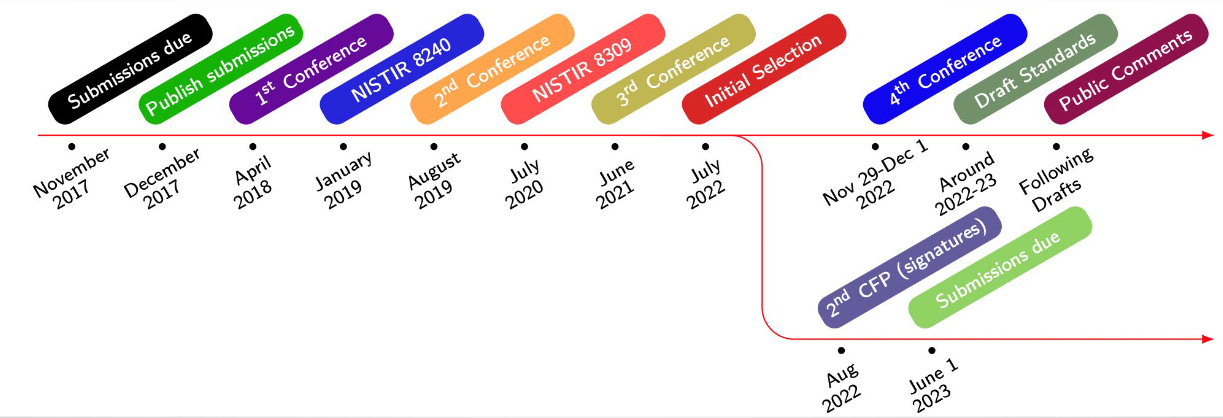
\includegraphics[width=1\linewidth]{Timeline.png}
        \caption{The latest timeline announced at the 4th PQC Standardization Workshop in 2023 \cite{moody_fourth}}
        \label{fig:timeline}
    \end{figure}

    \begin{table}[h!]
        \centering
        \begin{tabular}{cl}
             1801& Thomas Young's double-slit experiment kicks off field of quantum mechanics\\
     1935&Quantum entanglement discovered\\
     1935&Schr\"{o}dingers cat\\
     1955&Information science receives its name\\
     1965&Moore's law introduced\\
     1965&Stephen Weisner introduced conjugate coding\\
     1984&The BB84 protocol\\
     1994&Shor's algorithm\\
     1996&Grover's algorithm\\
     2015&NSA announcement\\
     2016&NIST announces PQC competition at PQCrypto\\
     2016&NIST releases NISTIR 8105, Report on PQC\\
     2016&NIST formal call for proposal\\
     2017&NIST deadline for submissions\\
     2017&IBM's 50-qubit quantum computer made\\
     2017&Round 1 algorithms announced\\
     2018&Intel's 49-qubit chip ``Tangle-Lake" made\\
     2018&Google's 72-qubit chip ``Bristlecone" made\\
     2018&NIST's first PQC standardization conference\\
     2019&Second round candidates announced\\
     2019&Deadline for updated packages for second round\\
     2019&Second PQC standardization conference\\
     2020&Third round candidates announced\\
     2020&Deadline for updated packages for third round\\
     2021&Third PQC standardization conference\\
     2022&Announcement of candidates to be standardized and fourth round candidates\\
     2022&Fourth PQC standardization conference\\
     2022&President of US releases NSM-8\\
     2023&Atom's 1180-qubit quantum computer made\\
     2023&President of US releases NSM-10\\
     2023&Three draft FIPS released for public comment\\
     2024&Fifth PQC standardization conference
        \end{tabular}
        \caption{A general timeline of quantum computing and NIST PQC standardization developments}
        \label{tab:qc_timeline}
    \end{table}
    
    \pagebreak
    
    \subsection{A Note on Polarizing Filters} \label{note:polarize}
    We have conceptualized qubits as photons with a spin in a particular direction or all possible directions in the case of superposition. If we were to compare a polarizing filter to a sieve, we might say that only photons with the same angle (or polarization) as the filter can get through the filter. But this is quantum physics, and in the case of qubits, it would be more accurate to say that if the polarization of the photon and filter match, all photons will get through; if they are opposite, none will get through; and if they are mismatch but not opposite (see Charles Bennett's definition of ``reliably distinguishable" in section \ref{superposition}), then a random number will get through the filter with the polarization possibly changed.

    \subsection{A Note on Symmetric Encryption}
    This paper has primarily focused on public key cryptography systems which are sometimes referred to as asymmetric key systems. An alternate type of encryption scheme is symmetric encryption. Research has indicated that these will be threatened by the development of a CRQC but not broken in the same way as public key systems, and as such, the increasing the length of keys for schemes such as AES and SHA-1/2/3 would be sufficient on the short term.
\pagebreak
\printbibliography
\end{document}
